\section{Introduction}

\begin{frame}{Trivia}

\end{frame}

\begin{frame}{Finding Oil -- Reverse Time Migration}
 \begin{figure}[!ht]
   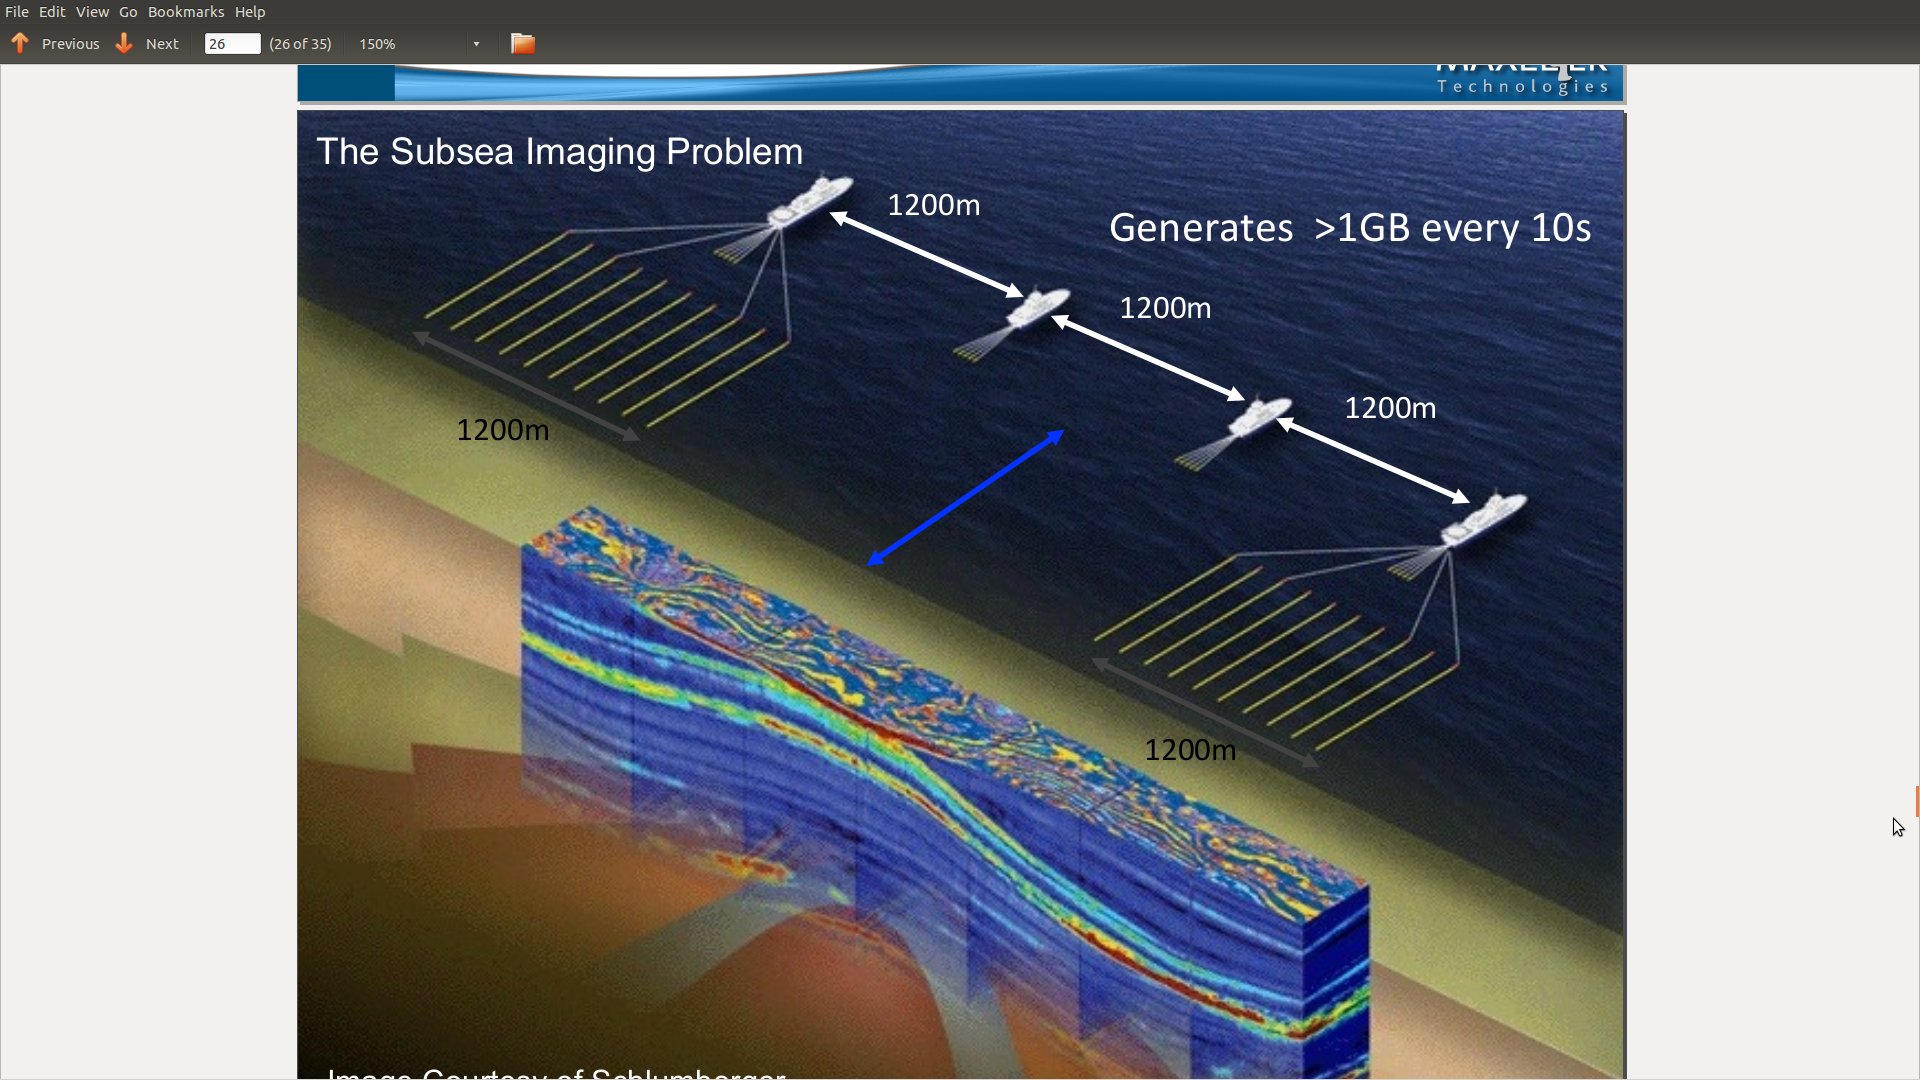
\includegraphics[scale=0.22, clip=true, trim=300 50 300 120]{figs/rtm-picture.png}
  \end{figure}
\end{frame}

\begin{frame}{High Performance Computing}
  \begin{columns}
    \column{.33\textwidth}
    \begin{figure}[ht]
      \centering
      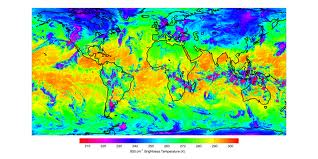
\includegraphics[scale=0.4, clip=true, trim=50 50 50 0]{figs/weather-forecasting.jpg}\\
    \end{figure}
    \column{.33\textwidth}
    \begin{figure}[ht]
      \centering
      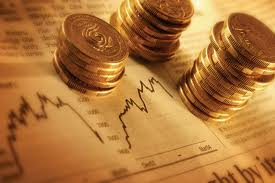
\includegraphics[scale=0.29, clip=true, trim=0 20 0 20]{figs/finance.jpg}\\
    \end{figure}
    \column{.33\textwidth}
    \begin{figure}[ht]
      \centering
      
\includegraphics[scale=0.25]{figs/ads.jpg}\\
    \end{figure}
  \end{columns}
  \vspace{0.5cm}

  \begin{beamerboxesrounded}{Requirements}
    \begin{itemize}
    \item Speed, Energy Efficiency, Productivity
    \end{itemize}
  \end{beamerboxesrounded}
  \vspace{0.5cm}

  \begin{beamerboxesrounded}{This Project}
    \begin{itemize}
    \item more \textbf{efficient} and more \textbf{productive} HPC
    \item first aspect-oriented compilation flow for dataflow HPC
    \item reproduce fastest, most efficient RTM dataflow design
    \item significant code reduction and less API calls
    \end{itemize}
  \end{beamerboxesrounded}
\end{frame}


\begin{frame}{More Efficient HPC -- Dataflow Engines}
\begin{itemize}
  \item FPGA based dataflow engines -- energy efficient HPC
 \begin{figure}[!ht]
   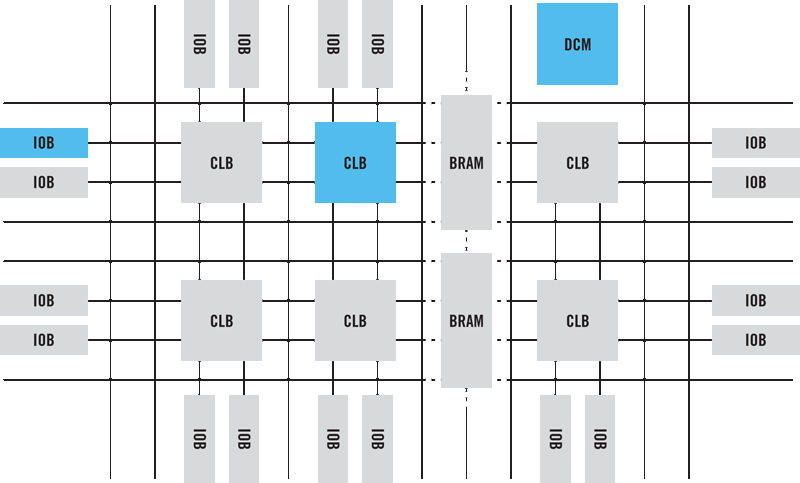
\includegraphics[scale=0.3, clip=true, trim=0 270 295 110]{figs/fpga-block-structure.png}
  \end{figure}
\hspace{0.25cm}
\item customisable hardware
  \begin{itemize}
  \item better performance and efficiency
  \item large design space
  \end{itemize}
\hspace{0.25cm}

\item \emph{The RTM porting to FPGA is the one that requires most
    effort.} Issues: development, debugging, portability. \footnote{Arraya-Polo, \emph{Assessing Accelerator-Based
HPC RTM, 2011}
}
\end{itemize}
\end{frame}

\begin{frame}
  \frametitle{Dataflow High-Performance Computing}
  \begin{figure}[!ht]
    \centering
    \def\svgwidth{0.9\linewidth}
    \input{figs/dataflow-both.pdf_tex}
  \end{figure}
\end{frame}

\begin{comment}
  \begin{frame}
    \frametitle{CPU vs Dataflow}
    \begin{columns}
      \begin{column}{.5\linewidth}
        \vspace{-1cm}
        \begin{figure}[!ht]
          \centering
          \def\svgwidth{\linewidth}
          \input{figs/compute-cpu.pdf_tex}
        \end{figure}
        \vspace{-0.5cm}
        \begin{itemize}
        \item Fast to develop
        \item Inefficient
        \end{itemize}
      \end{column}
      \begin{column}{.5\linewidth}
        \vspace{-1cm}
        \begin{figure}[!ht]
          \centering
          \def\svgwidth{\linewidth}
          \input{figs/compute-dfe.pdf_tex}
        \end{figure}
        \vspace{-0.5cm}
        \begin{itemize}
        \item Slow to develop
        \item Efficient
        \end{itemize}
      \end{column}
    \end{columns}
  \end{frame}
\end{comment}

\begin{frame}[fragile]
  \frametitle{Dataflow High-Performance Computing}
  \begin{comment}
    Developers must manually transform the original design to:
    \begin{enumerate}
    \item ensure I/O interface compatibility with host
    \item optimise resource usage by minimising operand width
    \item ensure result correctness by casting
    \item apply FPGA and dataflow specific optimisations
    \item replicate computational pipelines
    \end{enumerate}
    \vspace{0.5cm}
  \end{comment}
  \begin{beamerboxesrounded}{The Problem}
    Mixing optimisations with functional code makes it:
    \begin{itemize}
    \setlength{\itemsep}{10pt}
    \item harder to infer optimal designs (more constraints)
    \item harder to automate design space exploration
    \item impossible to re-target optimisations automatically
    \end{itemize}
  \end{beamerboxesrounded}
\end{frame}

\begin{comment}
  \begin{frame}[fragile]
    \frametitle{Decoupling Optimisations}
    \framesubtitle{Aspect-Oriented Design}
    \begin{beamerboxesrounded}{Aspect-Oriented Programming (AOP)}
      \begin{itemize}
      \item encapsulate cross-cutting concerns in aspect descriptions
      \item apply them at run-time to alter behaviour
      \item apply them at specified points (pointcut model)
      \end{itemize}
    \end{beamerboxesrounded}
    \vspace{0.75cm}
    \begin{beamerboxesrounded}{Aspect-Oriented Programming for Dataflow Engines}
      \begin{itemize}
      \item capture aspects of quality and their realisation
        \begin{itemize}
        \item speed, area, power, energy
        \item numerical accuracy, parallel computation
        \item optimisation, monitoring, debugging
        \end{itemize}
      \item use aspects to generate multiple variants of a design
      \end{itemize}
    \end{beamerboxesrounded}
  \end{frame}
\end{comment}

\begin{frame}[fragile]
  \frametitle{More Productive HPC -- Decoupling Optimisations}
  \begin{figure}[!ht]
    \centering
    \def\svgwidth{\textwidth}
    \input{figs/meng-aspect-weaving.pdf_tex}
  \end{figure}
\end{frame}
